
\chapter{Radiogoniometre}

 
\section{Module Montréal}

Le module Montréal comprends deux cartes électroniques : la carte principale qui est chargée de toutes les tâches relatives au traitement du signal reçu par les antennes et la carte destinée à l'affichage de la direction.

Les supports des cartes sont en résine époxy sur laquelle ont été apposée des pistes en cuivre en configuration mono-couche (les pistes ne sont présentes que sur une face de la plaque). Un étamage par dépôt chimique des piste a été réalisé pour les protéger de l'oxydation. L'ensemble de ces opération ont été effectuées à l'école avec l'aide de Mr. Gallou.
 
Le PIC18F4520 chargé de la majorité des traitements et le PIC12F675 ont été soudés sur la carte principale. Le PIC16F628A, chargé de l'affichage des LEDs a été soudé sur la carte d'affichage de direction. Le montage choisi pour ce dernier PIC permet de le désolidariser de la plaque afin d'effectuer les tests d'allumage des LEDs de direction.

L'ensemble des composants que nous avions a disposition (LEDs, condensateurs et résistances) ont été ensuite soudés sur les deux plaques. 

Par rapport au montage d'origine nous n'utiliseront pas le RS232. Toutefois, lors de la rédaction de ce rapport, il manque deux filtres sur la carte principale qui nous empêchent de valider son fonctionnement.


\section{Down converter}


\begin{wrapfigure}{r}{0.4\textwidth}
  
  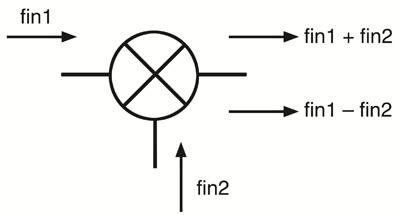
\includegraphics[width=0.4\textwidth]{mixer}
  \caption{schéma de fonctionnement d'un mixer}
\end{wrapfigure}


Le radiogoniomètre Montréal 3v2 fonctionne à une fréquence de 500Mhz. Sans modification il est impossible de l’utiliser entre 2.4Ghz et 2.5 GHz, bande de fréquence utilisée par les drones que nous souhaitons détecter. Nous avons donc cherché un moyen d’adapter ce radio-goniomètre aux fréquences souhaitées.

Une solution applicable à notre système est l'utilisation d'un down-converter. Ce composant reçoit deux entrées, le signal dont on veut changer la fréquence(RF) et un signal de fréquence fixe Df(LO). Le down-converter diminue la fréquence du premier signal de celle du second. La sortie(IF) correspond au signal modifié. Son principe de fonctionnement est illustré à la figure \ref{fig:mix}.



\begin{figure}[h]
  \centering
  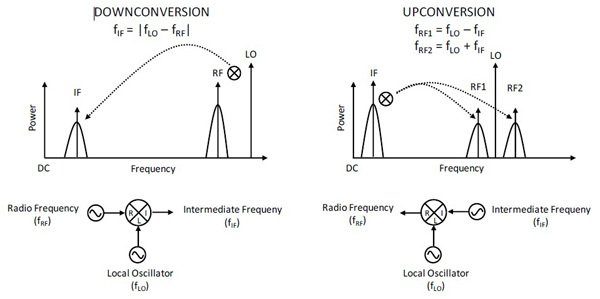
\includegraphics[width=\textwidth]{fonc_mixer}
  \caption{principe du fonctionnement d'un mixer}
  \label{fig:mix}
\end{figure}

On utilisera donc le down-converter pour abaisser la fréquence reçue par les antennes (2.4GHz) à la fréquence de travail du radio-goniomètre.

La fréquence du signal Df est donnée par un VCO (Voltage Controlled Oscillator ou oscillateur contrôlé en tension), le VCO reçoit en entrée une tension et donne en sortie une sinusoïdal de fréquence dépendante de la tension d’entrée. Le VCO étant très sensible, il est nécessaire de stabiliser la tension d’entrée et l’alimentation. On utilise donc un régulateur de tension qui amène une entrée stable. Le régulateur est un composant qui viendra limiter à une valeur seuil Vmax la tension qu'il reçoit en entrée si celle ci dépasse ce seuil. Dans le cas ou V < Vmax la sortie du régulateur sera égale à l'entrée.

Le VCO étant un composant actif et sensible aux variations dans sa tension d'alimentation, un second régulateur a été utilisé pour alimenter le VCO, toujours dans le but d’obtenir une fréquence stable ne variant pas pendant le processus. Il est en effet indispensable que cette fréquence reste fixe pour que l’effet doppler soit toujours visible et exploitable. Des fluctuation incontrôlées de la tension d'alimentation ou de la fréquence pourraient perturber la localisation.

Pour améliorer la mesure, il est utile de filtrer au maximum toutes le fréquences pouvant perturber la mesure et les différents bruits électromagnétiques. Ces phénomènes ont été atténués en positionnant en entrée du down-converter un filtre passe-bande qui permet de conserver uniquement la portion du spectre qui nous intéresse soit la bande située entre 2.4Ghz et 2.5Ghz.


\begin{figure}[h]
  \centering
  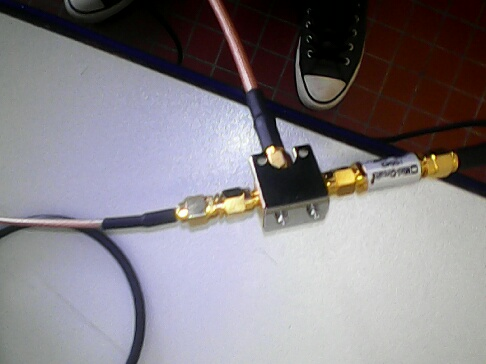
\includegraphics[width=0.5\textwidth]{down_converter}
  \caption{le down-converter et le filtre passe bande}
  \label{fig:down}
\end{figure}

A l’aide de ce montage on peut améliorer le signal en entrée pour qu'il puisse être traité par le radio-goniomètre.

%%% Local Variables: 
%%% mode: latex
%%% TeX-master: "../rapport"
%%% End: 
